\documentclass{article}
\usepackage{arxiv}
\usepackage[utf8]{inputenc} 
\usepackage{float}
\usepackage{listings}
\usepackage[T1]{fontenc}    
\usepackage{hyperref}       
\usepackage{url}            
\usepackage{mathtools}
\usepackage{amssymb,mathrsfs}
\usepackage{booktabs}       
\usepackage{amsfonts}       
\usepackage{dsfont}   
\usepackage[spanish]{babel}

\title{El Problema del Agente Viajero}
\author{
  Sandra del Mar Soto Corderi\\
  No. cuenta: 315707267
}
\date{}

\begin{document}
\maketitle

\section{Introducción}

El objetivo de este proyecto es implementar un sistema para resolver instancias del \textbf{Problema del Agente Viajero}\footnote{Del inglés \textit{Traveling Salesman Problem} (TSP)}, el cual dado un subconjunto de ciudades en un mapa, busca el camino más corto que pasa por todas ellas si es que existe.
Para lograr este objetivo, utilizamos la heurística de \textbf{Recocido Simulado} \footnote{Del inglés \textit{Simulated Annealing} (SA)} con la variante de \textbf{Aceptación Por Umbrales} \footnote{Del inglés \textit{Threshold Accepting} (TA)}.

Sea $S \subset V$ una instancia de TSP que se quiere resolver.
Para la resolución del TSP, primero se construyó una gráfica ponderada $G=(V,E)$ con las ciudades y sus respectivas conexiones (distancias entre las ciudades).
Esta gráfica no es completa, pero para facilitar la optimización la consideramos completa $G_s =(V_s, E_s)$, donde $V_s = S$ y $E_s= \{ (u,v) | u,v \in S \text{ y } u \not= v \}$ y la definimos con una función de peso aumentada para las aristas $w_s : E_s \to \mathds{R}^+$ definida como:
\[
  w_s(u,v) =
    \begin{cases}
      w(u,v)                   & \text{si }(u,v) \in E\\
      d(u,v) \times \max_d (S) &\text{en otro caso}\\
    \end{cases}
\]

donde $d(u,v)$ es la distancia natural entre dos vértices $u$ y $v$; y $max_d (S)$ será la \underline{distancia máxima} que existe entre los elementos de $S$ que están conectados en $G$.

La \underline{distancia natural} se utiliza para calcular la distancia natural entre dos elementos
de $S$ para de esta manera tener nuestra gráfica completa, se utilizarán las coordenadas de las
ciudades correspondientes. Su fórmula está definida por
\[
    d(u,v) = R \times C
\]
donde $R$ es el radio de la Tierra y $C$ está definida como $C = 2 \times \arctan(\sqrt{A},\sqrt{1-A})$. Con $A = \sin(\frac{lat(v)-lat(u)}{2})^2 + \cos(lat(u)) \times \cos(lat(v)) \times \sin(\frac{lon(v)-lon(u)}{2})^2$.

Esta definición se da de esta forma par que el sistema descarte las aristas que no están en $G$ para encontrar soluciones factibles más fácilmente.

Una \underline{solución de TSP} dada una instancia $S$, es cualquier permutación de los elementos de $S$ y se puede asegurar que estas soluciones son válidas para $G_s$. Dándonos así, dos tipos de permutaciones: las factibles y las no factibles. Decimos que es factible si y sólo si las aristas entre dos elementos consecutivos de la permutación existen en $E$. Si al menos una arista no existe, decimos que no es factible.


La optimización de TSP necesitará una \underline{función de costo} que evaluará ``qué tan buena (o no) es una solución'' y así se podrá decidir cuál es la mejor usando el criterio de comparación donde la evaluación con menor valor es la mejor. Para esto se va a normalizar la función de costo, pero para esto se necesitará un normalizador.

\underline{El normalizador}, como su nombre lo dice, normaliza la función de costo y nos dirá si una solución $S$ es factible si esta evaluada entre 0 y 1, y que una solución no factible se evalúe con un valor mayor que 1. Sea $L'$ los primeros $|S|-1$ elementos. La función se define como:
\[
\mathcal{N}(S) = \sum_{d \in L'}d
\]

La \underline{función de costo}, $f$ de una permutación $P = v_{\rho(1)}, \ldots, v_{\rho(k)}$ de los elementos de $S$ está definida como:
\[
    f(P) = \frac{\sum_{i=2}^{k} w_s(v_{\rho(i-1)}, v_{\rho(i)})}{\mathcal{N}(S)}
\]

Además de la función de costo, la optimización usa búsqueda local donde se deben conocer los $\underline{vecinos}$ de la solución de TSP. Dos soluciones son vecinas si intercambiando dos elementos de la primera se obtiene la segunda.

\subsection{Aceptación por Umbrales \emph{(Threshold Accepting)}}
Ahora hablaremos de la heurística: La heurística que se uso fue el \underline{recocido simulado}, la cual tiene su origen en la metalurgia, en el temple de metales. La idea de este es que si un metal se calienta a altas temperaturas y se le baja la temperatura abruptamente, el metal queda muy frágil, por otro lado si se baja la temperatura gradualmente, el metal se vuelve cada vez mas resistente. En pocas palabras, si se baja la temperatura lentamente, las propiedades del metal son mejores.

Viéndolo formalmente, dado un problema $\mathscr{P}$ de optimización y clasificado como NP-duro, sea $S$ el conjunto de posibles soluciones a una instancia de $\mathscr{P}$. Se supondrá que se tiene una función $f: S \to \mathds{R}^+$, (función objetivo), tal que $0 \leq f(s) \leq \infty$ para cualquier $s \in S$. Dadas $s,s'$ si $f(s) < f(s')$, entonces se considerará a la solución $s$ mejor que $s'$. En el proyecto se usará una variación del recocido simulado llamado aceptación por umbrales. La idea central de \underline{la aceptación por umbrales}, es que dada una temperatura inicial $T \in \mathds{R}^+$ y una solución inicial (obtenida de alguna manera),se busca de forma aleatoria una solución vecina $s'$ tal que $f(s') \leq f(s) + T$, y entonces actualizar $s$ para que sea $s'$, en este caso diremos que la solución $s'$ es \emph{aceptada}. Se continúa de esta manera mientras la temperatura $T$ es disminuida paulatinamente siguiendo una serie de condiciones: el proceso termina cuando $T < \epsilon$ (cuando se han generado un determinado número de soluciones aceptadas) o cuando otra serie de condiciones es satisfecha.

\section{Tecnologías usadas en el programa}
\begin{itemize}
	\item{ \textbf{Lenguaje de programación:} Kotlin 1.4.10. 
		
	Este proyecto se inició en el lenguaje de programación Rust pero por problemas de configuración y por cuestiones de tiempo, se decidió cambiar a un lenguaje ya conocido como es Java, pero ya que el profesor no es muy aficionado a Java, se buscaron alternativas y la mejor opción encontrada en ese momento fue Kotlin. Kotlin tiene una sintaxis muy intuitiva y permite usar todas las bibliotecas de Java.}
	\item {\textbf{IDE:} IntelliJ IDEA
		
	Es la IDE más popular para Java y es compatible con Kotlin, por lo que se usó}
	\item {\textbf{Sistema de construcción:} Gradle 6.7
		
	Al investigar la documentación de Kotlin, se mencionaba a Gradle y a Maven como las mejores opciones para usar como sistema de construcción. Gradle tenía el tutorial más corto, así como manejaba las dependencias más fácilmente que Maven, por ello se escogió.
	}
	\item {\textbf{Documentación:} dokkaHtml 1.4.10.2  
	
	Es el sistema de documentación oficial de Kotlin}
	\item {\textbf{Graficación:} Gnuplot 5.0 y Google Maps API}
	\item {\textbf{Insumos:} Los insumos (datos de entrada) fueron proporcionados por el profesor mediante una base de datos relacional \textit{SQL}. El sistema manejador de la base de datos utilizado es SQLite 3.16.2. El controlador del \textit{SMBD} es una biblioteca para Kotlin SQLite-JDBC 3.28.0.}
	\item {\textbf{Control de versiones:} Para mantener el control de versiones se utilizó Git 2.17.1 y el repositorio en línea se encuentra alojado en GitHub.}
\end{itemize}

\section{Diseño del programa}

\begin{figure}[H]
	\centering
	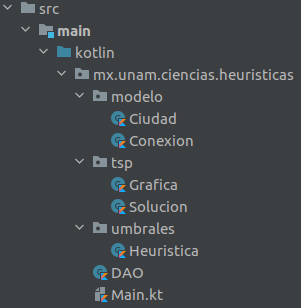
\includegraphics[scale=0.8]{imgs/estructura.png}
	\caption{Estructura de las clases del proyecto}
\end{figure}

El proyecto se hizo con un enfoque orientado a objetos, por la naturaleza del lenguaje escogido. 

Originalmente se iban a generar varias interfaces, pero al final se optó por un diseño más sencillo: El proyecto se dividió en tres paquetes: 
\begin{itemize}
	\item modelo
	
	En este paquete se crean los objetos que estaremos manejando en el proyecto y cuya información no cambiará, como son los valores de las ciudades y sus conexiones.
	\item tsp
	
	En este paquete tenemos todos los métodos o funciones necesarios para resolver el problema de tsp sin aplicar la heurística
	\item umbrales
	
	En este paquete tenemos los métodos o funciones necesarios para aplicar la heurística de recocido simulado con aceptación por umbrales al problema anterior.
\end{itemize}


A continuación se van a enlistar las clases usadas y lo que hace cada una:
\begin{itemize}
	\item {Ciudad.kt
		
		Esta clase almacena la información de las ciudades de nuestro problema, es decir, las coordenadas, nombre, id, población, de cada ciudad que se usará en el problema. Se declaró como una \emph{data class} de Kotlin, ya que este tipo de clases se dedican únicamente a almacenar información, lo que hace que al construir el objeto, hayan varios métodos ya implementados. Igualmente es necesario comentar que no se incluyó la implementación de getters y setters debido a que en Kotlin en la documentación mencionan que no son necesarios.
	}
	\item {Conexion.kt
		
		Esta clase es análoga a la de Ciudad en la cuestión que es una \emph{data class} donde guardamos las conexiones entre ciudades. Originalmente no se iba a usar este objeto, pero para facilitar el acceso a la base de datos con el DAO, se creó.
	}
	\item {Grafica.kt
		
		Esta clase es de las que cuentan con más métodos y es donde se realizan todas las funciones de la gráfica. Nuestra gráfica se representa como una matriz de adyacencia cuya forma de llenado sigue la definición de peso aumentado mencionado en la introducción. En esta clase se manejan los objetos de ciudad y conexion para obtener la información necesaria de acuerdo a la función. Cabe mencionar que para optimizar el tiempo en que corre el programa se agregó una función para obtener el peso de forma más directa, esta función optimiza la obtención del costo de la instancia una vez que se hace intercambio de índices al tomar las 4 aristas posibles de la gráfica que se ven afectadas con este intercambio y así obtener el nuevo costo restando los pesos de estas aristas eliminadas y la suma de agregar los nuevas aristas. Así obtenemos el peso durante las soluciones de forma constante y no lineal como sería en el caso de mandar a llamar a la función de costo de nuevo en cada caso.
	}
	\item {Solucion.kt
		
		Esta clase es bastante sencilla, ya que solo crea soluciones para el tsp, es decir invierte aleatoriamiente vecinos de la ruta para crear nuevas con la esperanza de que mejore. Esta clase originalmente iba a ir integrada con la clase de Grafica, pero era más limpio y fácil de comprender manejar los métodos de la clase heuristica con un objeto sencillo Solucion que con el objeto de una clase llena de métodos como es Grafica.
	
	}
	\item {Heuristica.kt
		
		Esta podría considerarse como la clase más ilustrativa del objetivo de este proyecto ya que es la que realiza el procedimiento de la heurística de recocido simulado con aceptación por umbrales. En pocas palabras el procedimiento que se sigue es obtener una temperatura con un valor lo suficientemente grande como para recorrer el espacio de búsqueda de forma rápida, esta temperatura se va disminuyendo al multiplicarla con un factor de congelamiento y mientras se enfría se van generando soluciones nuevas, de las cuales se toman las mejores. Los métodos de esta clase son la implementación los algoritmos que vienen descritos en el pdf llamado hoc que se encuentra dentro de la carpeta fuentes en este mismo directorio. Se había implementado un método que optimizaba los resultados, este método revisaba todos los vecinos de la mejor solución y tomaba el mejor de ellos, pero alentaba tanto al sistema que no se podían hacer las pruebas con muchas semillas.
	
	}
	\item {DAO.kt
		
		Esta clase funciona como nuestro Data Access Object, es la clase que se conecta con la base de datos directamente. Usamos un DAO por nuestro diseño basado en orientación a objetos y para mantener el patrón Modelo-Controlador. Normalmente los DAO no se aconsejan para aplicaciones donde el tiempo de ejecución importa pero es mucho más eficiente tener que hacer una o dos consultas a la base de datos mediante el DAO que hacer varias consultas dentro del modelo.
	}
	\item {Main.kt
		
		Este archivo no es una clase como tal, sino es el main donde se ejecuta el sistema. Lo que hace es tomar la lista de ciudades dada por el usuario con las cuales crea un objeto gráfica, este objeto gráfica manda a crear soluciones usando el rango de semillas proporcionado y manda a llamar a la heurística para mejorar la solución en los parámetros que se den. Al final se imprimen los costos de todas las mejores soluciones y se regresa la ruta de la mejor solución de todas.
	}
\end{itemize}

Para ver más detalladamente la implementación, favor de generar la documentación con dokkahtml.


\section{Resultados}

Probando diferentes semillas de un lote de 1000 semillas para ambas instancias de TSP (la de 40 y 150 ciudades), se logró encontrar una semilla para cada ejemplar de forma que se obtuvieran soluciones factibles y se tomó la mejor solución de todas. Para el caso de 40 ciudades el programa tuvo que ejecutarse por un aproximado de 5 horas mientras que para el caso de 150 tuvo que ejecutarse 16 horas.

El sistema tiene la cualidad de que cada vez que lo ejecutas aunque sea con la misma semilla, no te dará la misma función de costo, esto es por como se implementó la aleatoriedad en las soluciones dentro del programa. Por esa razón siempre se devuelve la ruta de la mejor solución, para que no se pierda. 

Los parámetros usados en el sistema de la heurística fueron cambiando de acuerdo a pruebas hechas con pocas semillas y las recomendaciones del profesor y la clase, después de encontrar mejores soluciones satisfactorias, los parámetros quedaron de la siguiente forma:
\begin{itemize}
\item Epsilon usada en la heurística de aceptación por umbrales 
0.00001
\item Epsilon usada en el algoritmo de obtención de la temperatura inicial
0.00001
\item Temperatura inicial del sistema 
8.0
\item Límite superior para las iteraciones al calcula un lote 
L = 2000
\item Factor de enfriamiento que determinará que tan rápido descenderá la temperatura T 
0.95
\item Porcentaje de soluciones vecinas
0.9
\item Valor de vecinos aceptados usados para calcular la temperatura inicial.
2000
\item Número máximo de iteraciones al calcular un lote 
L * 21
\end{itemize}

\subsection{Instancia con 40 ciudades}

Para la intancia de 40 ciudades tomaron los siguientes ids:

$[1,2,3,4,5,6,7,75,163,164,165,168,172,327,329,331,332,333,489,490,491,492,493,496,652,653,654, 656,657,\\ 792,815,816,817,820,978,979,980,981,982,984]$

Y se obtuvo un costo inicial de 3305585.454990047.

Después de ejecutar la heurística con 1000 semillas diferentes se obtuvieron soluciones mucho mejores, de las cuales se escogió la solución que generaba el menor costo, esta solución fue la generada por la semilla 635. 

Si se desea ver los costos que generaron las otras semillas durante esta ejecución, se pueden ver en el txt 40-1000-semillas.txt que se encuentra dentro del directorio resultado/resultadoIterandoSemillas

Al ejecutar el programa con 1000 semillas distintas vemos que en todos los casos se generaron soluciones factibles que oscilaban en el rango de 0.21-0.29 como valor de la función de costo

Usando la semilla \textbf{635} nos da los siguientes resultados:

Ruta: $[980, 327, 871, 331, 164, 984, 491, 492, 489, 4, 817, 978, 5, 6, 165, 3, 333, 981, 820, 332, 982, 816, 823, 7, 654, 490, 653, 656,\\ 2, 661, 657, 168, 1, 815, 496, 172, 163, 329, 493, 979]$

Costo: 0.21751778855705842

Así mismo se ejecutó el sistema de nuevo con la mejor semilla pero se guardaron los valores de sus evaluaciones y de sus mejores soluciones durante la ejecución, para poder graficarlas y compararlas. Podemos ver que el cambio en las soluciones tiene una mejor logística ya que en un punto baja rápidamente de valor y empiece a disminuir poco hasta que se acaba la temperatura.




\subsection{Instancia con 150 ciudades}
Con los identificadores de las ciudades:

$[1,2,3,4,5,6,7,8,9,11,12,14,16,17,19,20,22,23,25,26,27,74,75,151,163,164,165,166,167,168,169,171,172,173,174,\\176,179,181,182,183,184,185,186,187,297,326,327,328,329,330,331,332,333,334,336,339,340,343,344,345,346,347,\\349,350,351,352,353,444,483,489,490,491,492,493,494,495,496,499,500,501,502,504,505,507,508,509,510,511,512,\\520,652,653,654,655,656,657,658,660,661,662,663,665,666,667,668,670,671,673,674,675,676,678,815,816,817,818,\\819,820,821,822,823,825,826,828,829,832,837,839,840,871,978,979,980,981,982,984,985,986,988,990,991,995,999,\\1001,1003,1004,1037,1038,1073,1075]$

Se obtuvo un costo inicial de  6152051.625245281

Después de ejecutar la heurística con 1000 semillas diferentes se obtuvieron soluciones con costos mucho mejores, de las cuales se escogió la solución que generaba el menor costo, esta solución fue la generada por la semilla 727. 

Si se desea ver los costos que generaron las otras semillas durante esta ejecución, se pueden ver en el txt 150-1000-semillas.txt que se encuentra dentro del directorio resultado/resultadoIterandoSemillas

Al ejecutar el programa con 1000 semillas distintas vemos que no siempre se generaban soluciones factibles, pero se puede confirmar que más de la mitad fueron soluciones factibles. Esto se discutió en el seminario era normal debido a la cantidad de ciudades de la instancia. 

Usando la semilla \textbf{727} se obtuvieron los siguientes resultados:

Ruta: $[353, 990, 27, 333, 981, 3, 165, 988, 174, 4, 489, 817, 176, 668, 23, 352, 978, 6, 5, 1004, 351,991, 185, 22, 490, 653, 507, 2,\\ 656, 667, 184, 815, 9, 832, 661, 663, 657, 829, 1, 986, 508, 168, 505, 19, 839, 496, 182, 172, 173, 673, 665, 344, 654, 7, 823, 678,\\ 816, 187, 982, 14, 181, 345, 332, 26,820, 676, 163, 329, 509, 493, 979, 837, 995, 347, 499, 491, 492, 25, 501, 984, 1003, 349, 331,\\ 662, 8,
999, 674, 871, 343, 510, 660, 20, 825, 500, 985, 670, 350, 511, 327, 504, 334, 164, 11, 17, 444, 826, 840, 336, 980, 297, 828,\\ 12, 1038, 502, 340, 183, 75, 346, 171, 483, 652, 1075, 821, 512, 179, 671, 16, 520, 186, 675, 339, 151, 822, 1001, 74, 166, 658, 666,\\ 818, 655, 819, 330, 1073, 169, 1037, 326, 328,495, 167, 494]$

Costo: 0.14676221976439466

Así mismo se ejecutó el sistema de nuevo con la mejor semilla pero se guardaron los valores de sus evaluaciones y de sus mejores soluciones durante la ejecución, para poder graficarlas y compararlas. Podemos ver que el cambio en las soluciones tiene una mejor logística ya que en un punto baja rápidamente de valor y empiece a disminuir poco hasta que se acaba la temperatura.


\section{Conclusiones y Comentarios}

En conclusión, se hizo un proyecto que cumplía el objetivo y lo hizo de un forma bastante buena.

El tener que cambiar de un lenguaje a otro e iniciar desde cero el proyecto me atrasó bastante, lo que causó no pudiera refinar el diseño y la velocidad del sistema como quería. Además tuve varios problemas para usar gradle, lo que hacía que no pudiera probar lo que iba implementando. Igualmente tuve problemas para entender como funcionaba la heurística. A pesar de eso estoy satisfecha con mis resultados, mis mejores soluciones se acercaron bastantes a las del profesor y mi sistema no es tan lento como esperaba, se tardo demasiado con mis pruebas para las 1000 semillas, pero al ser tantas semillas no lo veo como algo malo.

En este proyecto estuve muchas veces en la encrucijada de si es mejor tener un sistema rápido o un sistema eficiente, en otro momento respondería siempre que es mejor un sistema eficiente, porque al final lo que queremos son buenas respuestas, pero cuando implementé una última optimización (hill descending) que hacía a mi sistema el triple de lento, me di cuenta que ganaría más tiempo probando diferentes parámetros con el sistema viejo que con este optimizado. Y así fue, obtuve casi las mismas soluciones probando con variaciones de la temperatura del sistema sin hill descending que esperando mucho más con la última optimización implementada. Por lo que opté no usar hill descending en la versión final.

Este proyecto me dio una mejor perspectiva para los próximos proyectos, los cuales haré con una mejor planeación. Me gustaría poder hacerlos en un lenguaje como Nim, Rust o C++ para que sean mucho más rápidos, aún así Kotlin fue bastante amigable y no me molestaría usarlo de nuevo. 

Fue muy divertido ver los cambios tan radicales de las soluciones cuando se implementó la heurística.

\begin{thebibliography}{9}
	\bibitem{tshgap}
	Día Juan A., Fernández E. A Tabu search heuristic for the generalized assignment problem. European Journal of Operational Research. 2001;132:22–38.
	  
	\bibitem{tabuglover}
	Glover F, Laguna M. Tabu search. S.L.: Kluwer Academic; 1993.  
\end{thebibliography}

Todas las fuentes que no son links se encuentran dentro del directorio fuentes ubicado en el directorio donde se encuentra este reporte.


\end{document}